\documentclass[11pt,a4paper]{article}

\usepackage{graphicx}
\usepackage[hmargin=1cm,top=1cm,bottom=1.2cm]{geometry}
\usepackage{xspace}  % smart spacing in custom commands
\usepackage{marvosym}  % for pictures and logos in title
\usepackage{ifsym}  % for pictures and logos in title
\usepackage{longtable}  % longtable that allows pagebreaks
\usepackage{array}
	\newcolumntype{C}[1]{>{\centering\arraybackslash}p{#1}}
\usepackage[utf8]{inputenc}  % allow use of french caracters
	\DeclareUnicodeCharacter{2010}{-}
\usepackage{enumitem}
	\setlist[itemize]{nosep,leftmargin=10pt}
	\setlist[itemize,1]{after=\vspace{-\baselineskip},label=\scriptsize\textbullet}
	\setlist[itemize,2]{after=\vspace{0cm},label=-}
\usepackage[usenames,dvipsnames]{xcolor}
	\definecolor{linkcolor}{HTML}{2000B0}  % blue-gray color for links
	\definecolor{gray}{gray}{0.3}  % gray for name
	\definecolor{headings}{HTML}{701112}  % dark red color for headings
\usepackage{hyperref}
	\hypersetup{colorlinks,breaklinks, urlcolor=linkcolor, linkcolor=linkcolor} % set up links and colors
\usepackage{fancyhdr}
	\pagestyle{fancy}
	\fancyhf{}  % clear all header and footer fields
	\renewcommand{\headrulewidth}{0pt}
	\renewcommand{\footrulewidth}{0pt}
	\fancyfoot[C]{\vskip-0.6cm\footnotesize\it\color{gray} References and additional information available upon request}

%% format of the section titles
\usepackage{titlesec}  % allows creating custom \section
	\newcommand{\secfont}{\color{headings}\scshape}
	\titleformat{\section}{\secfont\Large}{}{0.3cm}{}[\color{black}\titlerule]
	\titlespacing{\section}{0cm}{0.2cm}{0.2cm}  % spacing around titles (left, top, bottom)
	\titleformat{\subsection}{\secfont\large}{}{0.2cm}{}
	\titlespacing{\subsection}{0cm}{0.2cm}{0.2cm}

%% define better + and #
\def\Plus{\texttt{+}}
\def\cpp{C\Plus\Plus\xspace}
\newcommand{\Sharp}{{\settoheight{\dimen0}{C}\kern-.05em \resizebox{!}{\dimen0}{\raisebox{\depth}{\#}}}}

%% length of columns for tables
\newlength{\colone}
\newlength{\coltwo}
\settowidth{\colone}{Dec 2020 -- Dec 2020}
\setlength{\coltwo}{\textwidth} \addtolength{\coltwo}{-\colone} \addtolength{\coltwo}{-2\tabcolsep}

%% custom spacing
\setlength{\parindent}{0pt}  % no indent
\setlength{\LTpre}{0pt}  % no space around longtable
\setlength{\LTpost}{0pt}
\renewcommand{\arraystretch}{1.2}

%% shortcut commands
\newcommand{\cited}[1]{\par\footnotesize{~~--Cited: #1}}
\newcommand{\stars}[1]{\footnotesize{~-- #1 stars}}
\newcommand{\notes}[1]{{\small\color{gray}\itshape #1}}
\newcommand{\me}{{\bfseries M. Jacquet}}

\begin{document}

%----------------------------------------------------------------------------------------
%	title
%----------------------------------------------------------------------------------------
\begin{minipage}[t]{0.46\textwidth}
%% name and title
{\huge \bfseries \color{gray} Dr. Martin JACQUET}
\vskip0.4cm
{\large\bfseries Postdoctoral Researcher \par}
\vskip0.2cm
{\large\bfseries PhD in Robotics\par Engineer in Computer Sciences \par ~~and Applied Mathematics}
\end{minipage}
%% first info column
\begin{minipage}[t]{0.28\textwidth}
\vskip0.2cm
\flushright
\begin{tabular}{c|p{5cm}}
	\raisebox{0pt}{\Mobilefone}
		& \Plus33 (0) 6 47 63 60 50 \\
	\raisebox{0pt}{\Letter}
		& \href{mailto:martin.jacquet@posteo.net}{martin.jacquet@posteo.net} \\
	\raisebox{0pt}{\Letter}
		& \href{mailto:martin.jacquet@inria.fr}{martin.jacquet@inria.fr} \\
	\raisebox{-1pt}{
\includegraphics[height=0.3cm]{./images/scholar.png}}
		& \href{https://scholar.google.com/citations?user=CYG8yj4AAAAJ&hl=en&oi=ao}{Google Scholar page} \\
	\raisebox{-0.1cm}{
\includegraphics[height=0.35cm]{./images/github.png}}
		& \href{https://github.com/sedith}{Github page}
\end{tabular}
\end{minipage}
%% second info column
\begin{minipage}[t]{0.15\textwidth}
\vskip0.2cm
\begin{tabular}{c|p{5cm}}
	\raisebox{-4pt}{\textifsymbol{18}}
		& 4D all\'ee Verlaine,\par
		35000 Rennes\\
	\raisebox{-0.7pt}{
\includegraphics[height=0.3cm]{./images/bday.png}}
		& 28 septembre 1993\\
	\raisebox{-0.5pt}{
\includegraphics[height=0.3cm]{./images/car.png}}
		& Driving license\\
\end{tabular}
% \flushright 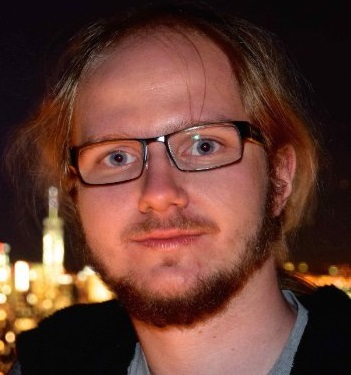
\includegraphics[scale=0.4]{./images/moi.jpg}
\end{minipage}
\vskip0.4cm

%----------------------------------------------------------------------------------------
%	experiences and education
%----------------------------------------------------------------------------------------
\section{Experiences \& Education}
\begin{longtable}{@{}C{\colone}p{\coltwo}@{}}
	Sep 2025 -- present \par
		\vskip0.5cm 
\includegraphics[height=0.8cm]{./images/inria.jpg}
	& {\bfseries Postdoctoral Researcher, at \href{https://www.inria.fr/fr/centre-inria-universite-rennes}{INRIA} - \href{https://team.inria.fr/rainbow/}{RAINBOW team}}, Rennes, France \par
	{Perception-based physical interaction with aerial robots} \par
	{\small
		With Dr. \href{https://marco-tognon-robotics.com/}{Marco Tognon}
		-- \href{https://anr.fr/Project-ANR-23-CE33-0013}{ANR-FlyHandyBot} project \par
		\begin{itemize}
			\item Nonlinear control for vision-constrained tasks
			\item Hybrid/Stochastic NMPC, MPPI
			\item Integration of onboard lidar-inertial state estimator
			\item ROS2, GenoM; Python, \cpp programming
		\end{itemize}
	}
\\
	2020 -- present \par
		\vskip0.3cm 
\includegraphics[height=1cm]{./images/ens.png} \par
		\vskip0.2cm 
\includegraphics[height=0.8cm]{./images/ntnu.pdf} \par
		\vskip0.1cm 
\includegraphics[height=0.5cm]{./images/n7.png}
	& {\bfseries Temporary Lecturer} \par
	{\small
	\begin{itemize}
		\item At \href{https://www.ens-rennes.fr/}{ENS Rennes} (M1, M2): 
			\begin{itemize}
				\item (2026) 28 hours of lectures and practicals -- Nonlinear control
				\item (2025) 6 hours of lectures -- Aerial robotics: modeling and control
			\end{itemize}
		\item At \href{https://www.ntnu.edu/en/home}{NTNU} (M1): 
			\begin{itemize}
				\item (2023) 10 hours of lectures and practicals -- ROS development
			\end{itemize}
		\item At \href{http://www.enseeiht.fr/en/index.html}{INP-ENSEEIHT} (L3, M1):
			\begin{itemize}
				\item (2021) 31 hours of seminars and practicals -- C programming, Android programming
				\item (2020) 21 hours of practicals -- Android programming
			\end{itemize}
	\end{itemize}
	}
\\
	Jul 2025 -- Aug 2025 & {Relocation to France, waiting for INRIA contract to start (unemployed)}
\\
	Feb 2023 -- Jun 2025 \par
		\vskip0.6cm 
\includegraphics[height=1cm]{./images/ntnu.pdf}
	& {\bfseries Postdoctoral Researcher, at \href{https://www.ntnu.edu/en/home}{NTNU} - \href{https://www.autonomousrobotslab.com/}{Autonomous Robots Lab}}, Trondheim, Norway \par
	{Perception-based control methods for collision-free navigation in unknown, complex and cluttered environments} \par
	{\small
		With Prof. \href{http://www.kostasalexis.com/}{Kostas Alexis}
		-- \href{https://cordis.europa.eu/project/id/101070405}{EU-Digiforest} project \par
		\begin{itemize}
			\item Deep learning for latent state/environment representations
			\item Interplaying neural methods with principled control methods (NMPC, CBF) for provable safety
			\item Software integration and Autonomy Stack development
			\item Neural world models, Reinforcement Learning
			\item ROS2, ROS, PX4; python, \cpp programming
			\item Robotics field-testing campaigns: hardware deployment, mission operator in forest environments
		\end{itemize}
	}
\\
	Nov 2025 -- Jan 2025 & {Postdoc position search, moving to Trondheim (unemployed)}
\\
	Jan 2019 -- Oct 2022 \par
		\vskip0.6cm 
\includegraphics[height=0.9cm]{./images/laas.png}
	& {\bfseries PhD in Robotics, at \href{https://www.laas.fr/en/}{LAAS-CNRS} - \href{https://www.laas.fr/en/teams/ris/}{RIS group}}, Toulouse, France \par
	{\bfseries Methods for Online Predictive Control of Multi-rotor Aerial Robots with Perception-driven Tasks subject to Sensing and Actuation Constraints} \par
	{\small	
		Advised by Prof. \href{https://r-franchi.eu/}{Antonio Franchi} -- \href{https://anr.fr/Projet-ANR-17-CE33-0007}{ARN-MuRoPhen} project \par
		\begin{itemize}
			\item Perception-constrained NMPC, Multi Aerial Robot Systems
			\item Active Perception methods, Observation uncertainty estimation
	     	\item ROS, GenoM; Python, Matlab and \cpp programming
	     	\item Involvement in the 2020 \href{https://www.mbzirc.com}{MBZIRC} robotics competition: perception-related software programming \par
			$\rightarrow${\bfseries Bronze medal} in the Grand Challenge competition
		\end{itemize}
	}
\\
	Jul 2018 -- Dec 2018 & {Personal travel experience (unemployed)}
\\
	Mar 2017 -- Jun 2018 \par
		\vskip0.4cm 
\includegraphics[height=0.9cm]{./images/laas.png}
	& {\bfseries Research Engineer at \href{https://www.laas.fr/en/}{LAAS-CNRS} - \href{https://www.laas.fr/en/teams/rap/}{RAP group}}, Toulouse, France \par
    {\small
		\begin{itemize}
			\item Collaborative project with the French Wine Institute (Gaillac) and Naïo Technology (Toulouse)
			\item Deep Learning-based detection of trunks and leaf diseases on wine images and videos
			\item Semantic segmentation, object detection, spatio-temporal classification
		    \item Python and \cpp programming, libraries Keras and TensorFlow
		\end{itemize}
	}
\\
	Oct 2016 -- Feb 2017 & {Unemployed}
\\
  	Summer 2016 \par
  		\vskip0.4cm 
\includegraphics[height=0.5cm]{./images/atos.jpg}
	& {\bfseries 6 months engineering internship at \href{https://atos.net/en/}{ATOS}}, Toulouse, France \par
    {\small
		Detection and tracking of icebergs in satellite images
		\begin{itemize}
			\item Semantic segmentation, classifications, temporal tracking
		    \item \cpp programming, web technologies (API development, SQL database, Docker, Kubernetes)
		\end{itemize}
	}
\\
	Summer 2015 \par
		\vskip0.4cm 
\includegraphics[height=1cm]{./images/irit.png}
	& {\bfseries 3 months research internship at \href{https://www.irit.fr/?lang=en}{IRIT}}, Toulouse, France \par
	{\small
		Search of symmetries for 3D-meshes compression
		\begin{itemize}
			\item Transposition of 2D algorithms in 3D for feature extraction (SIFT)
		    \item Statistical evaluation methodology
		    \item Matlab programming
		\end{itemize}
	}
\\
	Summer 2014
	& {\bfseries Work training period in a Japanese hotel, as a cleaning person} \par
	{\small Kamogawa Hotel Mikazuki, Kominato, Chiba, Japan}
\\
	2013 -- 2016 \par
		\vskip0.5cm 
\includegraphics[height=0.6cm]{./images/n7.png} \par
		\vskip0.2cm 
\includegraphics[height=0.6cm]{./images/polymtl.jpg} \par
	& {\bfseries Engineering degree, at \href{http://www.enseeiht.fr/en/index.html}{INP-ENSEEIHT}}, Toulouse, France \par
		\small{
			{\bfseries Computer sciences and applied mathematics department}
			\begin{itemize}
				\item Audiovisual data processing - Computer vision - 3D Modeling - Virtual Reality
				\item Mathematics - Statistics/Probabilities - Linear algebra - Optimization
				\item Computer sciences - Software programming
				\item School semester at \href{http://www.polymtl.ca/}{Polytechnique Montreal}, Canada; Courses in multimedia technologies \par
			    \item 2 months master's project : Building a 3D model of a scene from a flow of RGBD data
			\end{itemize}
		}
\\
	2011 -- 2013
		& {\bfseries Preparatory school, PSI* (Physics and Engineer Sciences)}\par
    	{\small Lycée Champollion, Grenoble, France}
\\
	2011
		&{\bfseries Scientific Baccalauréat}\par
		{\small Lycée Pierre Termier, Grenoble, France}
\end{longtable}


%----------------------------------------------------------------------------------------
%	publications
%----------------------------------------------------------------------------------------
\section{Scientific Publications}
% \begin{longtable}{@{}p{\colone}p{\coltwo}@{}}
% 	\small
% 	PhD Dissertation	& \me, \href{https://theses.fr/2022ISAT0021}{\it Methods for Online Predictive Control of Multi-rotor Aerial Robots with Perception-driven Tasks subject to Sensing and Actuation Constraints}
% \end{longtable} \par
\notes{Citation count and data as of 09/07/2026 \par
	Total citations: 180 \par
	h-index: 7 \par
}
\subsection{Journal Publications}
\begin{longtable}{@{}p{\colone}p{\coltwo}@{}}
	\href{https://www.scimagojr.com/journalsearch.php?q=18050&tip=sid}{IJRR}, 2025 \cited{1}
	& \me, M. Harms, K. Alexis, \href{https://doi.org/10.1177/02783649251401223}{\itshape Neural NMPC through Signed Distance Field Encoding for Collision Avoidance}
\\
	\href{https://www.scimagojr.com/journalsearch.php?q=21100900379&tip=sid}{RAL}, 2022 \cited{22}
	& \me, M. Kivits, H. Das, A. Franchi, \href{https://doi.org/10.1109/LRA.2022.3143218}{\itshape Motor-level N-MPC for Cooperative Active Perception with Multiple Heterogeneous UAVs}
\\
	\href{https://www.scimagojr.com/journalsearch.php?q=21100900379&tip=sid}{RAL}, 2021 \cited{40}
	& \me, A. Franchi, \href{https://doi.org/10.1109/LRA.2020.3045654}{\itshape Motor and Perception Constrained NMPC for Torque-Controlled Generic Aerial Vehicles} \par
		-- {\small{\bfseries Finalist for Best Paper Award} in Unmanned Aerial Vehicles at ICRA'21}
\end{longtable}
\notes{
	RAL is the IEEE reference for timely publications of major results in Robotics \par
	~~~~Impact Factor: 5.3 -- Journal Citation Indicator: 1.22 \par
	IJRR is among the two major venues for comprehensive Robotics publications \par
	~~~~Impact Factor: 5.0 -- Journal Citation Indicator: 1.36
}
%
\subsection{Conference Publications}
\begin{longtable}{@{}p{\colone}p{\coltwo}@{}}
	ICRA'25	\cited{8}
	& M. Harms, \me, K. Alexis, \href{https://doi.org/10.1109/ICRA55743.2025.11127368}{\itshape Safe Quadrotor Navigation using Composite Control Barrier Functions}
\\
	ICUAS'25 \cited{2}
	& N. Misyats, M. Harms, M. Nissov, \me, K. Alexis, \href{https://doi.org/10.1109/ICUAS65942.2025.11007827}{\itshape Embedded Safe Reactive Navigation for Multirotors Systems using Control Barrier Functions}
\\
	IROS'24	\cited{23}
	& M. Harms, M. Kulkarni, N. Khedekar, \me, K. Alexis, \href{https://doi.org/10.1109/IROS58592.2024.10802694}{\itshape Neural Control Barrier Functions for Safe Navigation} 
\\
	ICRA'24	\cited{20}
	& \me, K. Alexis, \href{https://doi.org/10.1109/ICRA57147.2024.10610572}{\itshape N-MPC for Deep Neural Network-Based Collision Avoidance exploiting Depth Images}
\\
	IROS'22	\cited{24}
	& G. Corsini, \me, H. Das, A. Afifi, D. Sidobre, A. Franchi, \href{https://doi.org/10.1109/IROS47612.2022.9981045}{\itshape Nonlinear Model Predictive Control for Human-Robot Handover with Application to the Aerial Case}
\\
	IROS'22	\cited{6}
	& \me, A. Franchi, \href{https://doi.org/10.1109/IROS47612.2022.9981643}{\itshape Enforcing Vision-Based Localization using Perception Constrained N-MPC for Multi-Rotor Aerial Vehicles}
\\
	AIRPHARO'21	\cited{5} & G. Corsini, \me, AE. Jimenez-Cano, A. Afifi, D. Sidobre, A. Franchi, \href{https://doi.org/10.1109/AIRPHARO52252.2021.9571053}{\itshape A General Control Architecture for Visual Servoing and Physical Interaction Tasks for Fully-actuated Aerial Vehicles}
\\
	ICRA'20	\cited{27}
	& \me, G. Corsini, D. Bicego, A. Franchi, \href{https://doi.org/10.1109/ICRA40945.2020.9197281}{\itshape Perception-constrained and Motor-level Nonlinear MPC for both Underactuated and Tilted-propeller UAVS}
\end{longtable}
\notes{ICRA and IROS are the two IEEE flagship conferences in Robotics}
%
\subsection{Book Chapters}
\begin{longtable}{@{}p{\colone}p{\coltwo}@{}}
	Springer, 2026 %\cited{0}
	& M. Camurri, E. Tomelleri, M. Mattamala, S. Barbas Laina, \me,
	\textit{et al.},
	% J. Behley, S. K.P. Kushwaha, F. Nan, N. Chebrolu, L. Freißmuth, M. Harms, M. V.R. Malladi, F. Yang, J. Frey, C. Cadena, M. Hutter, J. Schweier, K. Alexis, C. Stachniss, M. Fallon and S. Leutenegger,
	\href{https://TODO}{\itshape Digital Analytics and Robotics for Sustainable Forestry}, in \href{https://link.springer.com/book/9783032158116}{\itshape Recent Advances in Robotic Perception for Forestry}
\end{longtable}


%----------------------------------------------------------------------------------------
%	editorial services
%----------------------------------------------------------------------------------------
\section{Editorial services}
\begin{longtable}{@{}p{\colone}p{\coltwo}@{}}
	\bfseries Reviewer
		& Journals: 
			\href{https://www.scimagojr.com/journalsearch.php?q=19700182758&tip=sid}{Nature Communications},
			\href{https://www.scimagojr.com/journalsearch.php?q=95101&tip=sid}{T-RO},
			\href{https://www.scimagojr.com/journalsearch.php?q=18050&tip=sid}{IJRR},
			\href{https://www.scimagojr.com/journalsearch.php?q=21100900379&tip=sid}{RAL} \par
		Conferences: RSS, ICRA, IROS, ICUAS, ECC \\
	\bfseries Associate Editor
		& IROS (2026)
\end{longtable}


%----------------------------------------------------------------------------------------
%	supervising activities
%----------------------------------------------------------------------------------------
\section{Co-supervision of Master's Students}
\begin{longtable}{@{}p{\colone}p{\coltwo}@{}}
	Sep 2024 -- Dec 2024
		& {Nazar Misyats, ENS Rennes, France  \par
		\small{\itshape Development of a Safe Embedded Drone Controller based on Control Barrier Functions} \par
        Role: Topic definition, theoretical supervision, experimental hardware validation}
\\
	Jan 2024 -- Jul 2024
		& {Ask Espensønn Øren, NTNU, Norway \par
		\small{\itshape Multi-modal Learning-based Navigation} \par
        Role: Topic definition, technical supervision}
\\
	Jan 2024 -- Jul 2024
		& {Mathias Skogli, NTNU, Norway \par
		\small{\itshape Reinforcement Learning for Autonomous Safe Navigation in Dynamic and Cluttered Environments Exploiting Dynamics-Aware Embeddings of Depth Images} \par
        Role: Topic definition, technical supervision}
\\
	Jan 2020 -- Jul 2021
		& {Max Kivits, University of Twente, The Netherlands \par
		\small{\itshape Heterogeneous Cooperative Target Tracking using Nonlinear Model Predictive Control} \par
        Role: Topic definition, technical supervision, experimental hardware validation}
\\
	Jan 2020 -- Jul 2020
		& {Vamshi Kodipaka, University of Bourgogne, France \par
		\small{\itshape Vision based Multi-robot Tracking of Target with Aerial and Ground Robots} \par
        Role: Topic definition, technical supervision}
\end{longtable}


%----------------------------------------------------------------------------------------
%	open sourced releases
%----------------------------------------------------------------------------------------
\section{Maintained Open Source Software}
\begin{longtable}{@{}p{\colone}p{\coltwo}@{}}
	{\bfseries \href{https://ntnu-arl.github.io/unified_autonomy_stack/}{Autonomy Stack}}
		& Comprehensive Unified Autonomy Stack for Robots -- {\small Developer}\stars{210}
\\
	{\bfseries \href{https://ntnu-arl.github.io/sdf-nmpc/}{SDF-NMPC}}
		& Neural MPC for collision avoidance -- {\small Main developer, first author of related paper}\stars{47}
\\
	{\bfseries \href{https://github.com/ntnu-arl/composite_cbf}{CCBF}}
		& Composite CBF for collision avoidance -- {\small Main developer, author of related paper}\stars{12}
\\
	{\bfseries \href{https://github.com/ntnu-arl/PX4-CBF}{PX4-CBF}}
		& Embedded impl. of CCBF in \href{https://px4.io/}{PX4 Autopilot} -- {\small Developer, author of related paper}\stars{10}
\end{longtable}

\notes{
	All my papers also have an open-source implementation for reproducibility (not actively maintained)
}

%----------------------------------------------------------------------------------------
%	tech skills
%----------------------------------------------------------------------------------------
\section{Technical skills}
\begin{longtable}{@{}p{\colone}p{\coltwo}@{}}
	\bfseries Scientific
		& Neural Networks, Implicit neural representations \par
		Nonlinear optimal control \par
		Pose estimation, uncertainties, Kalman filtering \par
		Deep learning for image and video processing \par
		Mathematical modeling, physical parameters estimation \\
	\bfseries Languages
		& Python, {C\Plus\Plus}, C, Matlab \\
	\bfseries Programming
		& ROS2, ROS, GenoM, PX4, LateX, Git, Docker, Docker-compose \\
	\bfseries Librairies
		& PyTorch, OpenCV, Eigen \\
	\bfseries Hardware
		& Camera (calibration, data acquisition), Lidars, IMUs, Custom drones \& electronics
\end{longtable}


%----------------------------------------------------------------------------------------
%	languages
%----------------------------------------------------------------------------------------
\newpage
\section{Languages}
\begin{longtable}{@{}p{\colone}p{\coltwo}@{}}
	\bfseries French	& Native spealer \\
	\bfseries English 	& C2, fluent written and oral communication; {\sc Toeic} obtained in 2015 (940) \par
		Professional daily communication at work (working in international teams since 2019) \\
	\bfseries Spanish 	& High-school level (B1) \\
	\bfseries Japanese 	& Advanced Beginner \\
	\bfseries Norwegian & Beginner \\
	\bfseries Italian 	& Beginner \\
\end{longtable}


%----------------------------------------------------------------------------------------
%	misc
%----------------------------------------------------------------------------------------
\section{Various info}
\begin{longtable}{@{}p{\colone}p{\coltwo}@{}}
	% \bfseries Personal projects &
	% 	Video games prototyping \par
	% 	Hobby software development\\
	\bfseries Hobbies
		& Hobby software programming, cycling, brewing, tabletop role-playing, video games, cinema, photography, science-fiction
\end{longtable}

\end{document}
